%!TEX program = xelatex
\documentclass{article}
\usepackage{LaTeX-Submodule/template}

% Additional packages and macros
\usepackage{changepage} % Modify page width
\usepackage{multicol} % Use multiple columns
\usepackage{titlesec} % Modify section heading styles
\usepackage{textcomp, upquote} % Code block quotations support
\usepackage{calc} % Set exact

%% A4 page
\geometry{
	a4paper,
	margin = 10mm
}

%% Hide horizontal rule
\renewcommand{\headrulewidth}{0pt}

% Hide page numbers
\pagenumbering{gobble}

%% Multi-columns setup
\setlength{\columnsep}{4pt}

%% Paragraph setup
\setlength{\parindent}{0pt}
\setlength{\parskip}{0pt}

%% Customise section heading styles
\titleformat*\section{\raggedright\bfseries\large}
\titleformat*\subsection{\raggedright\bfseries}

\begin{document}
% Modify spacing
\titlespacing*\section{0pt}{0ex}{0ex}
\titlespacing*\subsection{0pt}{1ex}{1ex}
%
\setlength{\abovecaptionskip}{-5pt}
\setlength{\textfloatsep}{0pt}
%
\setlength{\abovedisplayskip}{1pt}
\setlength{\belowdisplayskip}{1pt}
%
\lstset{language=Matlab, upquote=true}
\lstset{morekeywords={randi, false, imshow, drawpolygon, polyarea, drawline, ones, imread, VideoWriter, XData, YData, getFrame, writeVideo, deg2rad, soundsc, resample, audiowrite, sind}}
%
\begin{multicols}{3}
    \section*{MATLAB}
    \lstset{belowskip=0pt, aboveskip=0pt}
    \begin{lstlisting}
% Function declaration
function [output1, ...]
    = function_name(input1, ...)
% Iterate over the vector v
for i = v ... end
% Repeat while condition is true
while condition ... end
% Execute first true alternative
if condition_1 ...
elseif condition_2 ...
else ... end
\end{lstlisting}
    \subsection*{Partial Fraction Decomposition}
    Given the LHS in the denominator, substitute the RHS\@.
    \begin{align*}
        \left(ax+b\right)^k & \to \frac{A_1}{ax+b} + \cdots + \frac{A_k}{\left( ax+b \right)^k}
    \end{align*}
    \begin{align*}
        \left(ax^2+bx+c\right)^k     & \to                                                   \\
        \frac{A_1x+B_1}{ax^2+bx+c} + & \cdots + \frac{A_k x+B_k}{\left( ax^2+bx+c \right)^k}
    \end{align*}
    \section*{Differential Equations}
    \subsection*{Mechanical Systems}
    \begin{equation*}
        \sum F = \odv{p}{t},\quad \sum M = I \odv[2]{\theta}{t}
    \end{equation*}
    where momentum \(p = mv\), moment \(M=Fx\) and inertia \(I=mr^2\).
    % \columnbreak
    \begin{align*}
        F_T & = \left( c - v \right) d_f & F_g & = -mg                         \\
        F_s & = -kx                      & F_f & = -b v^2 \text{ (or \(-bv\))}
    \end{align*}
    \subsection*{Electrical Circuits}
    \begin{align*}
        i = \odv{q}{t},\quad \sum v_{loop} = 0,\quad \sum i_{node} = 0
    \end{align*}
    \underline{Voltage drop across elements:}
    \begin{align*}
        v_R = iR,\quad v_C = \frac{q}{C},\quad v_L & = L \odv{i}{t}
    \end{align*}
    \subsection*{Separable ODEs}
    For \(\odv{y}{t} = p(t) q(y)\):
    \begin{equation*}
        \int \frac{1}{q(y)} \odv{y}{t} \odif{t} = \int p(t) \odif{t}.
    \end{equation*}
    \subsection*{Linear ODEs}
    For \(\odv{y}{t} + p(t)y = q(t)\), use the \textit{integrating factor}:
    \(I(t) = e^{\int p(t) \odif{t}}\), so that
    \begin{equation*}
        y(t) = \frac{1}{I(t)} \int I(t) q(t) \odif{t}.
    \end{equation*}
    \subsection*{Linearisation}
    \begin{align*}
        f(t)              & \approx f(t_0) + f'(t_0)(t-t_0)                                 \\
        f\bigl(y(t)\bigr) & \approx f\bigl(y(t_0)\bigr)                                     \\
                          & \phantom{\approx} + f'\bigl(y(t_0)\bigr)\bigl(y(t)-y(t_0)\bigr)
    \end{align*}
    \subsection*{Euler's Method}
    For \(\symbfit{y}' = \symbfit{f}(t,\: \symbfit{y})\):
    \begin{align*}
        \symbfit{y}_{n+1} & = \symbfit{y}_{n} + h\symbfit{f}(t_n,\: \symbfit{y}_n)
    \end{align*}
    \subsection*{Modified Euler's Method}
    \begin{align*}
         & \symbfit{y}_{n+1} =                                                                                                       \\
         & \symbfit{y}_{n} + \frac{h}{2}\left( \symbfit{f}(t_n,\: \symbfit{y}_n) + \symbfit{f}(t_{n+1},\: \symbfit{y}_{n+1}) \right)
    \end{align*}
    where \(\symbfit{f}(t_{n+1},\: \symbfit{y}_{n+1})\) is determined using Euler's method.
    \subsection*{Second-Order ODEs}
    \begin{equation*}
        ay'' + by' + cy = F(t)
    \end{equation*}
    \subsection*{General Solution}
    \begin{equation*}
        y(t) = y_H(t) + y_P(t)
    \end{equation*}
    \subsection*{Homogeneous Solution}
    \begin{equation*}
        y_H(t) = e^{\lambda t}
    \end{equation*}
    To solve for \(\lambda\), substitute the homogeneous form into the homogeneous ODE\@. \\
    \underline{Real distinct roots:}
    \begin{equation*}
        y_H(t) = c_1e^{\lambda_1 t} + c_2e^{\lambda_2 t}
    \end{equation*}
    \underline{Real repeated roots:}
    \begin{equation*}
        y_H(t) = c_1e^{\lambda t} + c_2 te^{\lambda t}
    \end{equation*}
    \underline{Complex conjugate roots:} \(\lambda = \alpha \pm \beta i\)
    \begin{equation*}
        y_H(t) = e^{\alpha x}\bigl( c_1\cos{\left( \beta t \right)} + c_2 \sin{\left( \beta t \right)} \bigr)
    \end{equation*}
    \subsection*{Particular Solution}
    \emph{See table below.}
    Substitute \(y_P\) into the nonhomogeneous ODE, and solve the undetermined coefficients.
    \subsection*{System of ODEs}
    Given \(\symbfit{y}' = \symbf{A} \symbfit{y}\),
    \begin{equation*}
        \symbfit{y}_H(t) = \symbfit{q}e^{\lambda t}.
    \end{equation*}
    \(\lambda_i\) are the eigenvalues of \(\symbfit{A}\) that satisfy
    \begin{equation*}
        \det{\left( \symbf{A} - \lambda\symbf{I} \right)} = 0.
    \end{equation*}
    \(\symbfit{q}_i\) are the associated eigenvectors that satisfy
    \begin{equation*}
        \left( \symbf{A} - \lambda_i \symbf{I} \right)\symbfit{q}_i = \symbf{0}.
    \end{equation*}
    \underline{For real distinct roots:}
    \begin{equation*}
        \symbfit{y}_H(t) = c_1\symbfit{q}_1e^{\lambda_1 t} + c_2\symbfit{q}_2e^{\lambda_2 t}
    \end{equation*}
    \subsection*{Higher-Order ODEs}
    \begin{equation*}
        y^{\left( n \right)} + a_1 y^{\left( n-1 \right)} + \cdots + a_{n-1} y' + a_n y = 0
    \end{equation*}
    Let \(y_1 = y\), \(y_2 = y'\), \dots, \(y_n = y^{\left( n-1 \right)}\)
    so that \(\symbfit{y}=\avec{y_1,\: y_2,\: \dots,\: y_n}\).
    Then \(\symbfit{y}' = \symbf{A} \symbfit{y}\), where
    \begin{equation*}
        \symbf{A} =
        \mqty[
        0      & 1        & 0        & \cdots & 0      \\
        0      & 0        & 1        & \cdots & 0      \\
        \vdots & \vdots   & \vdots   & \odifots & \vdots \\
        0      & 0        & 0        & \cdots & 1      \\
        -a_n   & -a_{n-1} & -a_{n-2} & \cdots & -a_1
        ]
    \end{equation*}
\end{multicols}
\begin{table}[H]
    \centering
    \begin{tabular}{c c}
        \toprule
        \(F(t)\)                                                               & \(y_P(t)\)                                                                \\
        \midrule
        a constant                                                             & A                                                                         \\
        a polynomial of degree \(n\)                                           & \(\displaystyle \sum_{i = 0}^n A_i t^i\)                                  \\
        \(e^{kt}\)                                                             & \(A e^{kt}\)                                                              \\
        \(\cos{\left( \omega t \right)}\) or \(\sin{\left( \omega t \right)}\) & \(A_0 \cos{\left( \omega t \right)} + A_1 \sin{\left( \omega t \right)}\) \\
        a combination of the above                                             & a combination of the above                                                \\
        linearly dependent to \(y_H(t)\)                                       & multiply \(y_P(t)\) by \(t\) until linearly independent                   \\
        \bottomrule
    \end{tabular}
\end{table}
\begin{multicols}{3}
    \section*{Probability}
    \subsection*{Events}
    \begin{gather*}
        \Pr{\left( A \right)} = \sum_{x\in A} p(x) \\
        \Pr{\left( A^C \right)} = \Pr{\left( \overline{A} \right)} = 1 - \Pr{\left( A \right)}
    \end{gather*}
    \subsection*{Unions}
    \begin{align*}
        \Pr{\left( A \cup B \right)} & = \Pr{\left( A \right)} + \Pr{\left( B \right)} \\
                                     & \phantom{=} - \Pr{\left( A \cap B \right)}      \\
                                     & = 1 - \Pr{\left( A^C \cap B^C \right)}
    \end{align*}
    \subsection*{Bayes' Theorem}
    \begin{equation*}
        \Pr{\left(B \;\middle|\; A\right)} = \frac{\Pr{\left( A \;\middle|\; B \right)}\Pr{\left( B \right)}}{\Pr{\left( A \right)}}
    \end{equation*}
    \subsection*{Disjoint Events}
    Events don't have outcomes in common.
    \begin{align*}
        A \cap B                   & = \varnothing \\
        \Pr{\left(A \cap B\right)} & = 0
    \end{align*}
    \subsection*{Independent Events}
    Outcome of events do not influence each other. Joint probability:
    \begin{equation*}
        \Pr{\left(A \cap B\right)} = \Pr{\left( A \right)}\Pr{\left( B \right)}
    \end{equation*}
    \subsection*{Dependent (Conditional) Events}
    Outcome of event depends on the outcome of the other. Joint probability of \(A\) given \(B\):
    \begin{equation*}
        \Pr{\left(A \;\middle|\; B\right)} = \frac{\Pr{\left( A \cap B \right)}}{\Pr{\left( B \right)}}
    \end{equation*}
    \subsection*{Total Probability}
    For disjoint events \(B_i\):
    \begin{align*}
        A                     & = \bigcup\limits_{i=1}^n \left( A \cap B_i \right) \\
        \Pr{\left( A \right)} & = \sum_{i=1}^n \Pr{\left( A \cap B_i \right)}
    \end{align*}
    \subsection*{Expectation}
    Average output or mean:
    \begin{equation*}
        \mu = \E{\left( X \right)}.
    \end{equation*}
    \subsection*{Variance}
    Measure of spread from the mean:
    \begin{equation*}
        \sigma^2 = \E{\left( X^2 \right)} - \E{\left( X \right)}^2.
    \end{equation*}
\end{multicols}
\begin{minipage}{126.1962963mm}
    \begin{multicols}{2}
        \section*{Probability Distributions}
        \subsection*{Discrete Random Variables}
        Has countably many outcomes. Distributed with a
        probability mass function \(p(x)\).
        \subsection*{Continuous Random Variables}
        Has an infinite number of outcomes. Distributed with a
        probability density function \(f(x)\).
        \begin{equation*}
            \Pr{\left( x_1 \leq X \leq x_2 \right)} = \int_{x_1}^{x_2} f(x) \odif{x}
        \end{equation*}
        \begin{equation*}
            F(x) = \Pr{\left( X \leq x \right)}
        \end{equation*}
        \subsection*{General Linear Combinations}
        \begin{align*}
            \E{\left( aX\pm b \right)}  & = a\E{\left( X \right)} \pm b                     \\
            \E{\left( aX\pm bY \right)} & = a\E{\left( X \right)} \pm b\E{\left( Y \right)}
        \end{align*}
        \begin{align*}
            \Var{\left( aX\pm b \right)}  & = a^2\Var{\left( X \right)}                    \\
            \Var{\left( aX\pm bY \right)} & = a^2\Var{\left( X \right)}                    \\
                                          & \phantom{=} + b^2\Var{\left( Y \right)}        \\
                                          & \phantom{=} \pm 2ab\Cov{\left( X,\: Y \right)}
        \end{align*}
        \begin{align*}
            \Cov{\left( X,\: Y \right)} & = \E{\left( XY \right)} - \E{\left( X \right)}\E{\left( Y \right)} \\
                                        & = \rho_{XY} \sqrt{\Var{\left( X \right)}\Var{\left( Y \right)}}.
        \end{align*}
        The correlation \(\Corr{\left( X,\: Y \right)}\) or \(\rho_{XY}\) is a constant that describes the statistical relationship
        between \(X\) and \(Y\). \(-1 \leq \rho_{XY} \leq 1\).
    \end{multicols}
    \begin{table}[H]
        \centering
        \begin{tabular}{c c c}
            \toprule
                                   & \textbf{Discrete}                              & \textbf{Continuous}                                    \\
            \midrule
            Valid probabilities    & \(0 \leq p(x) \leq 1\)                         & \(f(x) \geq 0\)                                        \\
            Cumulative probability & \(\sum_{u \leq x} p(u)\)                       & \(\int_{-\infty}^{x} f(u) \odif{u}\)                   \\
            Expectation            & \(\sum_{\Omega} xp(x)\)                        & \(\int_{\Omega} xf(x)\odif{x}\)                        \\
            Variance               & \(\sum_{\Omega} \left( x - \mu \right)^2p(x)\) & \(\int_{\Omega} \left( x - \mu \right)^2f(x)\odif{x}\) \\
            \bottomrule
        \end{tabular}
    \end{table}
\end{minipage}\hfill%
\begin{minipage}{62.39259259mm}
    \subsection*{Binomial (Discrete)}
    Probability of \(x\) successes out of \(n\) independent trials, each with chance \(p\).
    \subsection*{Poisson (Discrete)}
    Probability of observing \(x\) events over an interval \(t\), where events occur at an
    average rate \(\lambda\). \(\mu = \lambda t\).
    \subsection*{Exponential (Continuous)}
    The time \(t\) between events, where the events are independent and occur at an average rate \(\lambda\).
    \subsection*{Uniform (Continuous)}
    The probability of any value \(x\in\left[ a,\: b \right]\) is constant.
    \subsection*{Normal (Continuous)}
    Events occur more frequently near \(\mu\) and less frequently further away from \(\mu\).
    \subsection*{Standardised Normal (Continuous)}
    \begin{equation*}
        Z = \frac{X-\mu}{\sigma} \sim \mathrm{N}\left( 0,\: 1 \right)
    \end{equation*}
\end{minipage}
\begin{table}[H]
    \centering
    \begin{tabular}{c c c c c}
        \toprule
        \textbf{Distribution}                                      & \textbf{Probability}                              & \textbf{Cumulative Probability}           & \(\mu\)                  & \(\sigma^2\)                \\
        \midrule
        Binomial: \(X\sim \mathrm{bin}\left( n,\: p \right)\)      & \(\binom{n}{x} p^x \left( 1 - p \right)^{n - x}\) & \emph{See table above.}                   & \(np\)                   & \(np\left( 1-p \right)\)    \\
        Poisson: \(X\sim \mathrm{Pois}\left( \mu \right)\)         & \(e^{-\mu}\mu^x/{x!}\)                            & \emph{See table above.}                   & \(\lambda t\)            & \(\lambda t\)               \\
        Exponential: \(T\sim \exp{\left( \lambda \right)}\)        & \(\lambda e^{-\lambda t}\)                        & \(1 - e^{-\lambda t}\)                    & \(1/\lambda\)            & \(1/\lambda^2\)             \\
        Uniform: \(X\sim \mathrm{U}\left( a,\: b \right)\)         & \(1/\left( b-a \right)\)                          & \(\left( x-a \right)/\left( b-a \right)\) & \(\left( a+b \right)/2\) & \(\left( b-a \right)^2/12\) \\
        Normal: \(X\sim \mathrm{N}\left( \mu,\: \sigma^2 \right)\) & \(-\)                                             & \(-\)                                     & \(\mu\)                  & \(\sigma^2\)                \\
        \bottomrule
    \end{tabular}
\end{table}
\begin{minipage}{62.39259259mm}
    \section*{Sample Statistics}
    Given \(n\) samples \(x_i\):
    \begin{align*}
        \text{Mean:}     &  & \overline{x} & = \frac{1}{n}\sum_{i=1}^{n} x_i                                      \\
        \text{Variance:} &  & s^2          & = \frac{1}{n-1}\sum_{i=1}^{n} \left( x_i - \overline{x} \right)^2    \\
                         &  &              & = \frac{1}{n-1}\left( \sum_{i=1}^{n} x_i^2 - n\overline{x}^2 \right)
    \end{align*}
    \subsection*{t Distribution}
    The sample mean is distributed according to the t distribution where
    \begin{equation*}
        T=\frac{\overline{X} - \mu}{s/\sqrt{n}}\sim t_{n-1}
    \end{equation*}
    \begin{align*}
        \Pr{\left( T \leq t_{n-1,\: 1-\alpha/2} \right)} & = 1 - \frac{\alpha}{2} \\
        \Pr{\left( T > t_{n-1,\: \alpha/2} \right)}      & = \frac{\alpha}{2}
    \end{align*}
\end{minipage}\hfill%
\begin{minipage}{126.1962963mm}
    \begin{multicols*}{2}
        \subsection*{Confidence Intervals}
        Given the confidence level \(c\):
        \begin{equation*}
            c = 1 - \alpha.
        \end{equation*}
        The confidence interval for \(\overline{x}\):
        \begin{equation*}
            {CI}_{c} = \overline{x} \pm t_{n-1,\: 1-\alpha/2} \frac{s}{\sqrt{n}}.
        \end{equation*}
        \section*{Hypothesis Testing}
        Hypothesis testing assesses the likelihood of observing the sample \underline{if} the null hypothesis was true.
        \subsection*{Hypothesis}
        \begin{align*}
            H_0:\mu = \mu_0 \quad \text{vs} \quad H_1:\mu \neq \mu_0
        \end{align*}
        Generally there is no evidence supporting \(H_0\), but only evidence or lack of evidence for rejecting \(H_0\).
        \subsection*{Test Statistic}
        The measure of the distance that the proposed mean is from the sample mean:
        \begin{align*}
            T_{\text{test}} = \frac{\overline{x} - \mu_0}{s/\sqrt{n}}
        \end{align*}
        \subsection*{p-Value}
        Strength of evidence against \(H_0\). The \(p\)-value is the \(\alpha\) value that satisfies:
        \begin{equation*}
            \abs{T_{\text{test}}} = t_{n-1,\: 1-\alpha/2}.
        \end{equation*}
        \begin{align*}
            \Pr{\left( T \leq \abs{T_{\text{test}}} \right)} & = 1 - \frac{\alpha}{2} \\
            \Pr{\left( T > \abs{T_{\text{test}}} \right)}    & = \frac{\alpha}{2}
        \end{align*}
    \end{multicols*}
    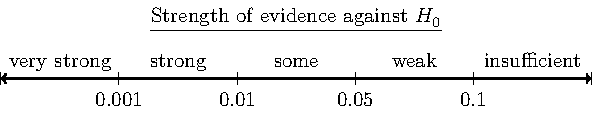
\includegraphics[width = \linewidth, keepaspectratio = true]{figures/p_values.pdf}
\end{minipage}
\begin{multicols}{3}
    \section*{Linear Regression}
    Given a set of \(n\) points \(\left( x_i,\: y_i \right)\) that are assumed to have a linear relationship,
    the model for \(y_i\) is
    \begin{equation*}
        y_i = \beta_0 + \beta_1 x_i + \varepsilon_i
    \end{equation*}
    where \(\varepsilon_i \sim \mathrm{N}\left( 0,\: \sigma^2 \right)\) is the residual.
    \(s\) (RMS error) gives an estimate for \(\sigma\) --- how close the data is to the model.
    \subsection*{Estimates}
    \begin{align*}
        T_{\text{test}}:\frac{\hat{\beta}_0 - \beta_0}{s_{\hat{\beta}_0}} \sim t_{n-2},\quad \frac{\hat{\beta}_1 - \beta_1}{s_{\hat{\beta}_1}} \sim t_{n-2}
    \end{align*}
    \subsection*{Inferences about \(\beta_0\) and \(\beta_1\)}
    \begin{align*}
        CI_c & = \hat{\beta}_0 \pm t_{n-2,\: 1-\alpha/2} s_{\hat{\beta}_0} \\
        CI_c & = \hat{\beta}_1 \pm t_{n-2,\: 1-\alpha/2} s_{\hat{\beta}_1}
    \end{align*}
    where \(s_{\hat{\beta}_0}\) and \(s_{\hat{\beta}_1}\) are the standard errors (SE) for \(\hat{\beta}_0\) and \(\hat{\beta}_1\).
    \(H_{0,\:\beta_0}:\beta_0=0\) tests whether the model crosses the origin.
    \(H_{0,\:\beta_1}:\beta_1=0\) tests whether the model is constant.
    \subsection*{R-squared}
    The percentage of the observed variance in \(y\) that is explained by the model.
    \subsection*{Residual Plots}
    Test the following two assumptions:
    \begin{enumerate}
        \item The relationship between \(X\) and \(Y\) is best modelled linearly
              --- clear indication of a non-linear trend suggests assumption is not valid.
        \item The variance of residuals is the same for all observations, (not affected by \(y_i\))
              --- uneven width of residual suggests assumption is not valid.
              This may lead to inaccurate inferences.
    \end{enumerate}
\end{multicols}
\end{document}
